\documentclass{standalone}
\usepackage{tikz,ifthen}
\usepackage{tkz-tab}
\usepackage{xcolor}
\usepackage{amsmath}
\usetikzlibrary{trees}
\begin{document}

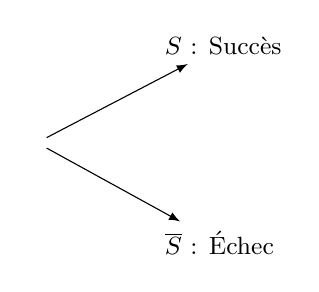
\begin{tikzpicture}[
		grow=right,
		level 1/.style={sibling distance=20mm},
		level 2/.style={sibling distance=20mm},
		edge from parent/.style={draw, -latex},
		every node/.style={font=\small}
	]

	\node {}
	child {
			node[below right] {$\overline{S}$ : Échec}
			% edge from parent node[above] {$P(S)$}
		}
	child {
			node[above right] {$S$ : Succès}
			% edge from parent node[below] {$P(\overline{S})$}
		};


\end{tikzpicture}

\end{document}
